\chapter{Inferring Interestingness of Tweets based on Information Flow Through the Network}


Mention:
\begin{itemize}
\item How this chapter builds upon network stuff in previous chapter
\item We hope to compare and contrast two better ways of predicting retweet volume \emph{and} interestness
\item What needs to be improved (speed, usability - more users with more followers etc.)
\item Why do improvements need to be made?
\item How is this useful, and how does first chapter relate to work done here?
\end{itemize}

Discuss:
\begin{itemize}
\item Does not use network to simulate tweets - instead uses a set of user features
\item Previous chapter shown how basic features can be used to generate a scale-free network, which is what twitter is
\item Use these features as input attributes of a new machine learning technique model.
\item This method does not use a network or model individual user decisions
\item Trained on a set of that particular user's tweets with the retweet outcome of integer type
\item A new tweet modelled with the regression outputs a retweet volume prediction without having to simulate the Tweet's travels through the network. 
\item Discuss about the machine learning approach used (logistic regression and how it works)
\item Talk about the 'binning' of retweet outcome volumes and its approaches (distribution dependent / independent, tables of precisions, etc.)
\item Link 'retweet volume' to 'retweet group size'
\end{itemize}

Mis-calculation errors when validating the interestingness predictions:
 - caused by non-authorisation to collect the data from Twitter (i.e. user has a protected account). Therefore we cannot build the test (or train data) successfully for these tweets
 - if an experimenter selected one of these Tweets, then we have to discard that timeline from our analyses.
 

In this chapter, we use the features surrounding both the social structure of Twitter and the Tweets that propagate within it to develop a methodology for deciding upon \textit{which} Tweets may be of specific interest, and also an introduction to inferring \textit{how} interesting the information is. The work does not take into account the relevance of a piece of information to a certain user, but instead the general interestingness level of the Tweet.\\
The work focuses on the difference between the raw popularity of a Tweet, demonstrated by its retweet activity, and how interesting the Tweet actually is to its recipients. While it has been shown that training a model with many Tweet features can be accurate in predicting how many times a Tweet might be retweeted \cite{zhu11}, here we focus on the notion of Tweet content beyond those static features. That is to say, when comparing the popularity of Tweets, that there is some content (either in the Tweet itself or in a webpage or image at a URL included in the Tweet) that makes that particular Tweet stand out and to cause \textit{affective stimulation} \cite{xu07} to viewers.\\
The focus of this work is in quantifying the interestingness of Tweets; that is, the universal relevance level of the information contained (or portrayed through links or media) in a Tweet. We infer this interest level by analysing the \textit{retweet volume} of Tweets in addition to their surrounding static features and the features of its source user and the network it propagates within. The retweet volume of a Tweet is defined as the total number of times that particular Tweet has been retweeted. \\
This paper considers only Tweets that have been retweeted using the `button' method, which is a single-click function on the Twitter website and its applications to carry out a retweet. Twitter users also sometimes imitate a retweet by copying the text of the original Tweet and prepending it with an ``RT'' followed by the original author's screen-name, which allows them to add annotations to the Tweet if they desire.\\ 
In this work, we introduce a method of calculating if a Tweet is interesting, or not. This is done on the basis of a comparison between a predicted retweet outcome for a particular Tweet and the \textit{observed} retweet volume of the Tweet. The method relies on the fact that the content of a Tweet is an important factor in retweet decisions, but avoids having to do much processing of the Tweet's text contents themselves (such as through natural language processing or sentiment analysis).\\
To determine \textit{how} interesting a particular Tweet is, we introduce an `interestingness score', which is based on the quantitative \textit{distance} between the real and predicted retweet volumes for a specific Tweet. The method and scoring is discussed in more detail later. If the interestingness score for Tweets can be determined and is known for a set of Tweets, then this method could be used as the basis for an information retrieval or delivery system, where relevant and interesting information can be shown to users without them having to know about it (e.g. follow the right set users) or search for it first.

\subsection{User Influence}
Of importance to this work is the difference between the retweet volume and the interestingness of a Tweet, and the fact that one does not necessarily indicate the other. The most obvious case in which this occurs is where there are influence discrepancies between users. For example, one of the most influential Twitter celebrities is Justin Bieber (@justinbieber), who, at the time of writing, has nearly 40 million worldwide followers and achieves an average of around 50-120 thousand retweets per Tweet. His Tweets currently rarely receieve less than 40,000 retweets. \\
Average Twitter users generally attract a couple of hundred followers and would normally receive very few (if any) retweets per Tweet. A particularly interesting Tweet from such a user may be retweeted around 5-20 times (though this depends entirely on the level of influence of a user and their number of followers).\\
It is therefore apparent that an uninteresting Tweet from Justin Bieber could get retweeted 50,000 times and an exceptionally interesting Tweet from a less-influential user may get 30 retweets, and that the retweet volume, in this case, really isn't indicative of the \textit{interestingness} of the particular Tweet.\\
Of course, this brings about the notion of information relevance, and the fact that a Tweet could be very boring or irrelevant to one user, and very interesting to another. In this work we focus on \textit{global} (or `average') interest, where retweet scores and predictions are made for the general case. It is our belief that Tweets that are retweeted more than expected within their authors' local networks (relative to the authors' own regular output) are also likely to be of interest to a wider audience.


\section{Interestingness Scores}
As discussed, our proposed process for deciding upon a Tweet's interest level involves conducting comparisons between the number of times a Tweet has been retweeted and the \textit{predicted} retweet volume of the Tweet. The premise behind this is that there is something beyond the static features of a Tweet (e.g. whether, or not, the Tweet contains a URL, the length of its content, the influence of its author, etc.) that causes a specific Tweet to be more interesting than another with precisely the same feature set.\\
The retweet count of a specific Tweet is returned, at the time of writing, as part of a standard call to v1.1 of the Twitter REST API, and includes the total number of times that the original Tweet was retweeted using the button retweet method.\\
Essentially, our method follows these basic steps:
\begin{enumerate}
\item Obtain and extract contextual information on a given Tweet, $t$,
\item Generate predictions on the retweet volume for $t$,
\item Compare the predicted values to the \textit{observed} retweet count of $t$,
\item Make inferences based on this difference between the predicted and observed values.
\end{enumerate}
We use Bayesian Network classifiers, trained on a set of Tweet and environmental features, in order to make predictions on a Tweet's retweet volume. In this work we consider two of these classifiers for making predictions for each Tweet; one trained on the Tweet's source user's own Tweets and another trained on a `global' corpus of Tweets (a larger dataset of Tweets from many source users). Thus, we obtain two retweet volume predictions for each Tweet.\\
For a Tweet, $ t $, we define the observed (or `real') retweet outcome to be $ T_O(t) $, the predicted outcome using the global corpus model to be $ T_{P_G}(t) $, and the predicted outcome using $t$'s author's user-centric corpus model to be $ T_{P_U}(t) $. The scores for $t$'s actual outcome compared to the predicted outcome using the global and user-centric models, $ TS_G(t) $ and $ TS_U(t) $ respectively is calculated thus;

\[
\begin{array}{cc}
 TS_G(t) = \frac{T_{P_G}(t)}{T_O(t)} &  TS_U(t) = \frac{T_{P_U}(t)}{T_O(t)} 
\end{array}
\]

This provides a positive score where;

\[
TS_G(t) \text{,  } TS_U(t)
	\begin{cases}
		> 1		&	\text{indicates } t	\text{ is interesting} \\
		\leq 1	&	\text{indicates } t	\text{ is non-interesting}
  \end{cases}
\]

$ | TS_G(t) - 1 | $ represents \textit{how} interesting (or non-interesting) $t$ is and $TS_{Avg}(t)$ denotes the mean of its user and global score.\\
This method relies on collecting retweet data from Twitter and involves taking a snapshot of Tweets at one stage during their lifetime. Since Tweets do not decay (unless they are deleted by their author), they can be found and retweeted by users at any time after their composition. In this work, we assume that the significant portion of retweet activity has already occurred for the Tweets that have been collected. Indeed, \cite{kwak10} carried out temporal analyses on retweet behaviour and discovered that, on average, 75\% of the retweets of a particular Tweet occur within one day and that 50\% of retweets take place within one hour of the Tweet being posted.\\
Based on this, to ensure that the retweet count mostly reflected the `final' retweet count, only Tweets more than one day old were considered for experimentation.


\subsection{`Twitter is a Memepool'}
The term `meme' was defined to be a ``unit of cultural transmission'' \cite{dawkins76} and the notion of memetics is an analogy to biological genetics. Unlike genes, memes are entirely non-physical and represent a cultural idea or other human-based behaviour. \\
Genes survive and are passed on through \textit{replication}, and this replication occurs more frequently and efficiently when they are more suited to their environment. A gene's genome is the set of information that represents, in its entirety, the features that make up that particular gene (such as eye colour, height, some aspects of personality, and so on).\\
Memes are similar in that they contain a set of features, such as the wordings of a phrase or their relevance to other cultural aspects, which cause them to be less or more likely to be replicated in different environments. For example, an Internet meme relating to the Star Wars movies would likely have a greater chance of reproduction (through reposting, discussion, etc.) in an environment of sci-fi fanatics than when amongst more mixed groups.\\
The meme is a useful analogy for the work in this paper, since it also helps outline the way in which Tweets are replicated within Twitter. Like a meme, a Tweet has a specific set of features (the text it contains, any hashtags, the inclusion of mentions, and so on) and it exists within an environment consisting of a set of interconnected users on the Twitter social graph. A particular Tweet would generally have a greater chance of being reproduced, through retweeting, in certain networks than others. Tweet features are similar to the \textit{genome} of a gene and the features of the network the Tweet exists in (i.e. the users that receive and have the opportunity to assist in a Tweet's propagation) form the \textit{environment}.
\\ 
More:
\begin{itemize}
\item Gene is a physical entity containing information and instructions. It is a unit of genetic inheritance (i.e. offspring typically have a mashup of the genes of the parens)
\item The result of the data held by a gene (the genome) means that organisms with certain genes are able to reproduce and survive more than other organisms containing different genes.
\item Thus the gene is able to replicate under certain gene- and environmental-centric conditions.
\item A meme is similar to  gene but is non-physical. They are a unit of cultural inheritance (an idea, phrase, behaviour, etc.).
\item Like genes, memes are able to survive better when their features (\textit{menome}) are suited to the meme's environment. In such environments, the meme is able to be shared and replicated more efficiently and frequently.
\item A Tweet, again, is similar to both. A Tweet itself has many features (the text of the Tweet, the time of its origin, its length, etc.) and their environment, the Twitter social structure, has features (namely the users that belong to it and the way they are connected) which may facilitate the replication (i.e. Retweet) of the Tweet.
\item A Tweet existing in different social structures will have different Retweet patterns, which is what we want to show in this chapter.
\item Thus tweetfeatures = genome, userfeatures=environment
\end{itemize}


\section{Retweet Volumes as Nominal Attributes}
In order to try and improve the accuracy of the model at predicting retweet volume outputs, a nominal output attribute would be better than a real one. Predicting a continuous numeric value could render inaccurate results and calculating the cut-off points at which to mark as the upper- and lower-bounds for the output based on the inputs would raise difficulties.
\\
Instead, the retweet outcomes were to be `binned' into several categories which would be determined on the fly based on the outcomes present in the training data.\\

In the global model and each of the user models, the retweet volume was trained as the \textit{outcome} feature.  Accurately predicting continuous values is a challenge for many machine learning algorithms due to the way the model is built around the features. To assist with this in our experimentation, the retweet outcomes were `binned' into nominal outcome categories.\\
The binning algorithm needed to be dynamically based on the distribution of retweet outcomes so that each bin was of a roughly equal size.


\subsection{Binning the Retweet Outcomes}
Describe the different methods (linear, distributed 1, distributed 2), and their advantages/disadvantages, with examples showing the graph of 
what the bins look like.
\\
Focus on the distributed 2 example, and why this is better.
`Requested' bin number not usually the same number as what is actually returned (due to large numbers of smaller retweet groups).
\\
Pseudocode\\

In \cite{webberley11} it was shown how the general distribution of retweet volumes forms a long tail with a very high proportion of single retweets and for which the frequency drops off considerably for larger retweet volumes. As a result, linearly binning the outcomes would reduce the number of feature instances for higher retweet outcomes and thus cause the Bayesian Network classifiers to be considerably less accurate.\\
The binning algorithm that was used involved calculating the projected size of each bin from on the total number of feature instances and the desired target number of bins. The bins were then filled accordingly, such that each retweet volume frequency would only appear in one bin. For example, The feature instances with zero retweets would all appear in the first bin, no matter how many there were. Instances with larger retweet volumes would then typically share a bin with instances with similar retweet volumes. Each bin `range' (i.e. the range of retweet volumes of instances contained in the bin) represents a nominal category of the retweet volume outcome in the Bayesian Network, and each feature set instance is associated with precisely one outcome category.\\
Since the binning algorithm is dynamic, the bin sizes and ranges vary from dataset to dataset. As a result, the categories in each user-based dataset are different from one another, reflecting the different number of retweets that each author's Tweets are likely to receive. 

\subsection{Varying Bin Sizes}
Number of bins: explain how accuracy worsens as bin number increases.
\\


\section{Techniques Used}
For the work presented in this chapter, various techniques and approaches were used for handling the data and for generating the scores. The most notable are now assessed in this section.

\subsection{Machine Learning}
Explain about Machine Learning, its uses, techniques and how this is useful.
\\
Talk about how it was used in previous chapter, but that more in depth here.
Bayesian Network

\subsubsection{Classification Performance}
Compared several types of classifiers (show table comparing accuracy, etc. of different types)
\\
Explain that Bayesian Network is best (quick, accurate)

\subsubsection{Training Results}
Playing with Weka to improve the prediction performance (i.e. different number of bins, different features)

\subsection{Crowdsourcing}
Crowdsourcing is a technique often employed by companies and researchers to collect large amounts of data from a (often large) distribution of people or devices. Examples of this in practice include the use of surveys and user-contributed reviews (such as in Google Maps).\\
In this paper we use Amazon's Mechanical Turk service as a method for crowdsourcing interestingness validations from many people, who are known as Mechanical Turk Workers (MTWs) 


\section{Experimentation}
In this section we describe the stages involved in making interestingness inferences of Tweets based on their individual retweet behaviour. We start by discussing how the data was collected and how the information was then processed. We go on to illustrate how we employed our Bayesian Networks and the features we extracted for training them in order to make the retweet predictions. We finish by discussing how we then infer the Tweet interestingness and how this was validated.

\subsection{Data Collection}
In March 2013, a random walk was carried out through the Twitter social graph using Twitter's REST API, originating with one of this paper's author's Twitter account. Each step of the walk involved focusing on one Twitter user, collecting information on that user, and then selecting a random follower of that user. This follower then became the focus of the next step.\\
At each step, a set of the most recent Tweets from the current user were collected. The number of Tweets returned by the Twitter API differed from user to user, based on their recent Tweet-posting frequency, though usually a few hundred Tweets were yielded. In addition to their Tweets, we also collected information on the user itself and on a sample subset (up to 100, if they exist) of its friends and followers. We used a sample instead of collecting information on \textit{all} of a user's friends and followers so that we could maximise the efficiency of our method in terms of data collection. It also meant we had a snapshot of an additional 200 users in the author's local network to give the classifier a notion of the activity of this local network both upstream and downstream from the author.\\
This gave a dataset containing around 241,000 Tweets from 370 unique Twitter users and, of those Tweets, around 90,000 were cases where the retweet volume was greater than zero. The dataset was split into two datasets: a training set (90\%) and the testing set (10\%). The original dataset was split in such a way as to allow all Tweets belonging to one particular user to exist in only one of the two smaller datasets. The training set was used to train a model, as described below, and was then discarded from the rest of the experimentation.

\subsection{Data Corpora}
As discussed in the methodology section, we are interested in producing \textit{two} predictions for each Tweet; one when compared to the global set, and another from comparisons to the rest of that user's Tweets. Therefore, a new dataset was formed for each user in the testing dataset which contained the Tweets only from that particular user. For the remainder of this section, the testing dataset is the \textit{global} corpus of Tweets, and each of the individual user datasets are known as \textit{user} corpora.\\
The Bayesian Network was chosen as our classifying algorithm to produce the predictions as it was suitable for the data types of the Tweet and user features and was also found to perform efficiently in terms of precision and recall across the outcome predictions when carrying out test cross-validations against itself. The prediction precision weighted across the outcome categories was calculated to be around 70\% in cross-validation tests on the training dataset features.

\subsection{Features}
To train the Bayesian Network model, a series of new features were harvested. Generally, each of these features fell into one of two categories; user features and tweet features.
\\
The Tweet features follow the same ideas as the features used in the previous chapter: static, generally binary features that describe the structure of the Tweet. The user (or `network')  features are related more to the \emph{network} to which the Tweet belongs.\\

Features were extracted from the Tweet and user data to train the Bayesian Networks. Each Tweet is represented by an \textit{instance} of feature sets specific to that Tweet (and its author, if appropriate). In each instance the outcome feature is the retweet volume, which is categorised using the technique discussed later.\\
Since some features are static among Tweets from the same user (for example, a user's follower count), a different feature set is used to train the user models and the global model, as described below.

\subsubsection{Features for the global corpus model}
A total of 31 features were used to train the model classifier from the global data corpus.

\begin{table}[h]\footnotesize
\begin{center}
\begin{tabular}{ c | l | c }
	 Feature category	& Feature & Feature data type \\
	 \hline
	 \hline 
	& mention & \{True, False\}\\
    & Tweet length & real (numeric)\\
    & url & \{True, False\}\\
  	& hashtag & \{True, False\}\\
  	Tweet & positive emoticon & \{True, False\}\\
  	(`genome')& negative emoticon & \{True, False\}\\
  	& exclamation mark & \{True, False\}\\
  	& question mark & \{True, False\}\\
  	& starts with `RT' & \{True, False\}\\
  	& is an @-reply & \{True, False\}\\
  \hline                        
	& follower count & real (numeric)\\
    & friend count  & real (numeric)\\
	Author & verified account & \{True, False\}\\
	& status count & real (numeric)\\
	& listed count & real (numeric)\\
  \hline
  	&  max. follower count & real (numeric)\\
	&  min. follower count & real (numeric)\\
	&  avg. follower count & real (numeric)\\
    Network &  max. friend count & real (numeric)\\
	(`environment') &  min. friend count & real (numeric)\\
	&  avg. friend count & real (numeric)\\  
	&  avg. status count & real (numeric)\\  
  	& proportion verified & real (numeric)\\  
  \hline  
\end{tabular}
\end{center}
\caption{Features used to train the model from the global data corpus}
\label{table:globalfeatures}
\end{table}

The features used to train the global model are outlined in Table \ref{table:globalfeatures}. The network features apply to both the followers and friends retrieved for each author. For example, the first feature of this category, `max. follower count', represents two features referring to the maximum follower count observed in the sample of the author's followers and in the sample of the author's friends. \\
While Tweet features are permanent after the Tweet has been created, the author and network features are dynamic in that the social graph is of a constantly altering structure as links are formed and broken between users. However, in this work, we assume that the changes to these features are not significant over the Tweets collected for each user and try to minimise this by only considering recent Tweets of each user.

\subsubsection{Features for individual user models} 
The 10 Tweet features were used for training each user-based Bayesian Network to reduce redundancy in the model since the author and network features would be the same across all of the Tweets from one user.



\subsection{Making predictions and inferring Tweet interestingness}
The global and user models were then trained using the features to produce one global model and one user model for each unique author in the testing dataset, as described above.\\
To produce the global predictions, $ T_{P_G} $, each Tweet in the testing database was evaluated against the global model, which output a predicted value for the bin that Tweet is predicted to belong to.\\
The user predictions, $ T_{P_U} $ were calculated in the same way: each Tweet in the testing dataset was evaluated against the model based on the Tweet's author.\\
Each Tweet then each had two retweet volume predictions. The upper bound of the binned category assigned to each prediction was compared to the \textit{observed} retweet count to produce the two interestingness scores, $ TS_G $ and $ TS_U $, as discussed earlier.


\subsection{Planning the Result Validation}
To assist in validating the interestingness scores produced for the Tweets, tests were required in which humans would be responsible for also assessing how interesting they feel the Tweets were. The predicted interesting Tweets could then be compared to the Tweets chosen as interesting through human judgement.\\
For this stage of the experimentation, certain Tweets (and users) were removed from the dataset to be tested by the humans. Since the Tweet data was collected using a random walk through Twitter, there was no governance over the content of the text in this data. Therefore, users who frequently used offensive or non-English (since the Tweets were to be validated by English-speaking individuals) language had their Tweets removed from the test set. In addition, individual `@-replies' (Tweets starting with the `@' symbol) were also stripped from the test set since these usually denote conversations on Twitter between two or more users and are unlikely to convey any interest to outsiders.


\subsubsection{Validating the Results}
In this context, MTWs have no connection to the Tweets in the dataset, and are random users of Amazon's Mechanical Turk who decide to take the job on. Collecting the validation data in this way, and instead of using a small set of people, means that we can collect a diverse opinion on Tweet interestingness from people whom the Tweets will have varying relevance to. This helps reinforce the notion of \textit{global} interest levels, where Tweets can be interesting to a large number of users.\\
The human validations were carried out such that the MTWs were presented with questions, each of which consisting of five different Tweets from one specific author. Each question asked that the MTW select the Tweets they consider to be the most interesting of the group and that they must select at least one. MTWs were paid \$0.05 for each question they answered and there were 91 unique MTWs in total who responded to the questions.\\
The tests were under the conditions of a randomised controlled trial, such that each Tweet was assessed in three different contexts (i.e. each Tweet would appear in three different questions alongside four randomly chosen other Tweets) and that each question would be responded to by three different MTWs.\\
To represent the validation for this ongoing work, 750 Tweets were selected, at random, from the stripped testing dataset and were organised by user to ensure that Tweets only appeared in questions alongside other Tweets from the same author. Since each Tweet was required to appear in three different questions and each question consisted of 5 unique Tweets, this resulted in a total of 450 unique questions, each of which was answered by three different MTWs.

\subsection{Validation Results}
From the 450 questions asked of the MTWs, 325 questions had responses where the response was chosen with a confidence of two-thirds or greater. Since MTWs had the opportunity to choose more than one Tweet to be the most interesting, 349 Tweets (the subset of all tested Tweets), denoted as $T$, were selected as sufficiently interesting. Tweets selected from individual questions by only one of the assessing MTWs for that question were discarded.

\subsubsection{General Performance}

\begin{figure}[h]
\centering{
\begin{tikzpicture}
\begin{semilogyaxis}[
    symbolic x coords={[0-1), [1-2), [2-3), [3-4), [4-5), [5-100)},
        ylabel=Proportionate frequency,
		xlabel=$TS_G(t)$,
        %enlargelimits=0.15,
        %legend style={at={(0.5,-0.15)},anchor=north,legend columns=-1},
        legend pos=north east,
        legend style={nodes=right},
        ybar,
        bar width=7pt,
        legend entries={ Chosen Tweets ($T$),  All Tested Tweets}
        ]
   \addplot[plot 0,bar group size={0}{2}]
        coordinates {([0-1),76.30057803) ([1-2),7.514450867)  ([2-3),4.335260116) ([3-4), 1.445086705) ([4-5), 2.023121387) ([5-100), 6.936416185)};
        \addplot[plot 1,bar group size={1}{2}]
        coordinates { ([0-1),80.94365552) ([1-2),6.596426935)  ([2-3),3.710490151) ([3-4), 1.099404489) ([4-5), 0.961978928) ([5-100), 4.634448007)};
        
\end{semilogyaxis}
\end{tikzpicture}
}
\caption{Proportionate frequency distribution of global scores in the entire test set compared to only those in the subset $T$.}
\label{fig:hist}
\end{figure}

In the subset $T$, our method predicted 140 Tweets to have $TS_G(t) > 1$ and 80 Tweets where $TS_U(t) > 1$.  These results were validated by the MTWs in that they agreed that all Tweets $t \in T$ where $TS_{Avg}(t) > 1$ were interesting in 60\% of cases, with the performance of the global scores, $TS_{G}(t)$, achieving 65\% precision. The user scores, $TS_{U}(t)$, were less accurate and yielded a precision of around 55\%.\\
In addition, we show how the proportionate frequency of Tweets with higher values of $TS_G(t)$ is greater in the subset $T$ than in the entire set tested with the MTWs (Figure \ref{fig:hist}). This also demonstrates that Tweets with low global scores ($0 \leq TS_G(t) < 1$) are more frequent in the entire test set than in the subset $T$.

\subsubsection{Per-Question Performance}
\begin{figure}[h]
\centering{
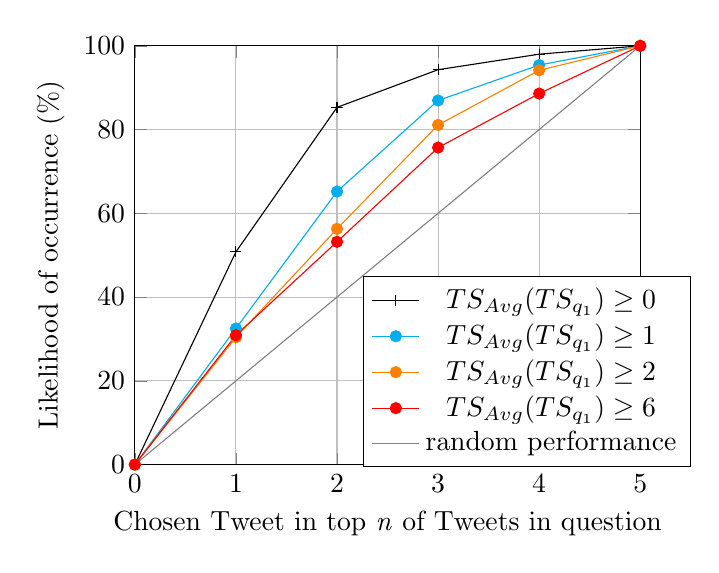
\begin{tikzpicture}
 \begin{axis}[
        xlabel=Chosen Tweet in top \textit{n} of Tweets in question,
        ylabel=Likelihood of occurrence (\%),
        grid = major,
        legend entries={$TS_{Avg}(TS_{q_1}) \geq 0 $, $ TS_{Avg}(TS_{q_1}) \geq 1 $, $TS_{Avg}(TS_{q_1}) \geq 2 $, $TS_{Avg}(TS_{q_1}) \geq 6 $, random performance},
        %legend style={nodes=right},
		%legend pos=south east,
		legend style={at={(1.1,0.45)}},
		%legend style={nodes=right, at={(0.6,0.5)},anchor=north},
		xmin=0, xmax=5,
		ymin=0, ymax=100	,
		width=8cm
		]
	\addplot[mark=+,black] plot coordinates {
        (0,0) (1,50.8) (2,85.3) (3,94.3) (4,98) (5,100)
        };
        
	\addplot[mark=*,cyan] plot coordinates {
        (0,0) (1,32.5) (2,65.2) (3,86.95) (4,95.4) (5,100)
        };
    \addplot[mark=*,orange] plot coordinates {
       (0,0) (1,30.4) (2,56.3) (3,81.1) (4,94.15) (5,100)
    };
    \addplot[mark=*,red] plot coordinates {
        (0,0) (1,30.9) (2,53.2) (3,75.7) (4,88.6) (5,100)
    };
    \addplot[gray] plot coordinates {
        (0,0) (1,20) (2,40) (3,60) (4,80) (5,100)
    };
\end{axis}
\end{tikzpicture}
}
\caption{The probability of the MTW's chosen Tweet's $TS_{Avg}(t)$ being in the top \textit{n} of Tweets for that question while varying the minimum allowed maximum Tweet score of the question.}
\label{fig:score-dist}
\end{figure}
Analyses were also conducted on the performance of the predictions on a per-question basis. Hereafter, a question, $q \in Q$, is defined as a set of Tweets where;
\[ q = {t^q_1, t^q_2, t^q_3, t^q_4, t^q_5} \]
and
\[ |q| = 5 \]

For conducting these question-based analyses, each question's five Tweets were ranked in order of ascending mean interestingness score such that $TS_{Avg}(t^q_1) \geq TS_{Avg}(t^q_2) \geq ... \geq TS_{Avg}(t^q_5)$. We then calculated the number of times the MTWs chose a Tweet that appeared in the top $n$ of the ranked list of Tweets, as shown in Figure \ref{fig:score-dist}.\\
In this figure, we vary the minimum allowed value of $TS_{Avg}(t^q_1)$ (the highest Tweet score in question $q$) to show how detecting more interesting Tweets was more accurate when the range of scores in each question is more disparate. We show, for cases in which $TS_{Avg}(q_1) \geq 1$, that the likelihood of the MTWs choosing one of our two most highly ranked Tweets of the question using the interestingness predictions is around 66\% and the chance that they choose one of the top three ranked Tweets is 87\%.

\subsubsection{Probability of Selection}

\begin{figure}[h]
\centering{
\begin{tikzpicture}
\pgfplotsset{every axis plot/.style={line width=2pt}}
 \begin{axis}[
        xlabel=$ x $,
        ylabel=$P(\text{t chosen} : TS_G(t) > x)$ ,
        grid = major,
        height=5.2cm, width=8cm,
        xmin=0, xmax=4
       ]
	\addplot+[smooth, mark=none]  table {6.Chapter3/data/cum-dist-score.dat};
\end{axis}
\end{tikzpicture}
}
\caption{The probability that Tweet $t$ is chosen given that $TS_G(t)$ is greater than a given value, $x$.}
\label{fig:score-cum-dist}
\end{figure}

Finally, we show that the probability of MTWs deciding a Tweet $t$ is interesting becomes higher as the value of $TS_G(t)$ increases. \\
In Figure \ref{fig:score-cum-dist}, although we exclude cases of Tweets with $TS_G(t) > 4$ to reduce noise (due to fewer samples), a significant increase in probability is observed, particularly in the interval 0-1 representing the range of Tweets that are uninteresting (fewer observed retweets than predicted) to `as expected' (observed retweet volume is equal to predicted). It is also illustrated that, from this initial work, Tweets with a predicted interestingness score of 3 or more are not significantly different from one another in terms of their `real', human-judged, interestingness. However, more work will be carried out towards this in the future so that more accurate research can be done on Tweets with scores of greater then 3 in this context.


\section{Further Analyses}
The interestingness scores have been validated in terms of there being recognition that they can signify interesting Tweets. This section will now continue onto some deeper analyses of the results in order to show \textit{how} it is able to work.

\subsection{Discerning Interesting Information from Noise}
In this subsection, the human-selected interestingness selection will be assessed. Of particular interest is the likelihood of humans agreeing on an interesting piece of information and the properties of the Tweet scores in questions when agreements \textit{are} made. \\
For this, analyses were made into the \textit{disparity} of scores for Tweets. That is, the range of scores of Tweets in a particular question and the effect this has on human decision in deducing interesting information.

\begin{table}[h]\footnotesize
\begin{center}
\begin{tabular}{ c | c | c | c }
	 Num. confident answers in $q$& min. $d^{Avg}(q)$ & max. $d^{Avg}(q)$ & avg. $d^{Avg}(q)$ \\
	 \hline
	0 & 0 & 846 & \textbf{17.6} \\
	> 0 & 0 & 1445 & 32.1 \\
	1 & 0 & 1445 & \textbf{34.3} \\
	> 1 & 0 & 4 & 0.647 \\
	> 2 & 0 & 0.55 & 0.204
\end{tabular}
\end{center}
\caption{Absolute $TS_{Avg}(t)$ disparity of questions with varying number of confident answers made. Entries in \textbf{bold} are used to highlight interesting values.}
\label{table:score_disparities}
\end{table}

The absolute Tweet score disparity for a question, $q$, is defined as $d(q)$. For example, for a disparity of average scores, this is calculated thus;

\[ d^{Avg}(q) = \max(TS_{Avg}(q)) - \min(TS_{Avg}(q)) \]

Table \ref{table:score_disparities} shows how the values for $TS(q)$ vary for questions with differing numbers of confident answers. A confident answer, as mentioned previously, is one where at least two MTWs have agreed on an interesting Tweet.\\
The data shows that the average $TS(q)$ is around double in cases where a question is answered with precisely one confident answers than in cases where there are no confident answers made. This indicates that a wider scale of interestingness in a question is useful for humans for picking out the content they'd prefer to read. If several pieces of content are more similarly interesting (or, as the case may be, uninteresting), then it becomes more difficult for an agreement to be made on which information is the \textit{most} interesting.\\
In addition, the average score disparities in cases where multiple confident answers were selected are very low. This helps to reinforce the notion that pieces of information that are very similar in terms of interest level make it hard for users to decide on the \textit{most} interesting. Indeed, in questions where this is the case, MTWs have selected, and agreed on, multiple Tweets.

 \begin{figure}[h]
\centering{
\begin{tikzpicture}
\pgfplotsset{every axis plot/.style={line width=2pt}}
 \begin{axis}[
        xlabel=Average $d^{Avg}(q)$,
        ylabel=Cumulative probability of a confident selection being made,
        grid = major,
        height=7.5cm, width=13cm,
       ]
	\addplot+[mark=none]  table {6.Chapter3/data/cum-question-disparity.dat};
\end{axis}
\end{tikzpicture}
}
\caption{The probability of a confident selection being made for question $q$ with varying $d(q)$.}
\label{fig:cum-question-disparity}
\end{figure}

To take this further, it is demonstrable that the probability of a confident selection being made for a particular question, $q$, increases as $TS(q)$ also increases (Figure \ref{fig:cum-question-disparity}.  Thus, this reinforces the notion that people find it easier to discern interesting information when compared to \textit{un}-interesting information. This, too, is highlighted in Table \ref{table:score_disparities_2}, in which it is shown that amongst \textit{all} questions (i.e. not only questions that have been confidently-answered) the score disparity is much smaller between Tweets that were selected than the score disparity for the entire question. \\
This is particularly the case in which there are a few Tweets which have similarly high scores amongst Tweets which collectively have \textit{lower} scores. Therefore, selecting confidently from the few Tweets with the similar scores become difficult, but it is demonstrated that these at least are \textit{more} interesting than the ones that weren't selected.\\

\begin{table}[h]\footnotesize
\begin{center}
\begin{tabular}{ l || c | c | c }
	   & $TS_G(t)$ &  $TS_U(t)$ &  $TS_{Avg}(t)$\\
	 \hline
	$TS_d(q)$ & 62.4 & 4.7 & 33.3\\
	$TS_{d_C}(q)$ & 35.3 & 3.1 & 19.0\\
	\hline
	Ratio & 57\% & 66\% & 58\%
\end{tabular}
\end{center}
\caption{Score disparity comparison between selected Tweets of question $q$ and \textit{all} Tweets in $q$ when using the three different Tweet scores as metrics}
\label{table:score_disparities_2}
\end{table}

For example, this data shows that, on average, the global score disparity for selected Tweets of a question, $q$, was only around 57\% that of the entire disparity of $q$.